% NeurIPS-style formatting: matches Google/DeepMind paper layout
\documentclass[10pt]{article}

\usepackage[utf8]{inputenc}
\usepackage[T1]{fontenc}
\usepackage{amsmath,amssymb,amsfonts}
\usepackage{graphicx}
\usepackage{booktabs}
\usepackage{microtype}
\usepackage{hyperref}
\usepackage{tikz}
\usetikzlibrary{shapes.geometric, arrows.meta, positioning, fit, calc}
\usepackage{mathptmx}  % Times-like font (NeurIPS standard)
\usepackage{nicefrac}

% NeurIPS page geometry: 5.5in x 9in text block, US Letter
\usepackage[letterpaper]{geometry}
\geometry{
  textwidth=5.5in,
  textheight=9in,
  top=1in,
  left=1.5in,
  headheight=12pt,
  headsep=25pt,
  footskip=30pt
}

\setlength{\parindent}{0pt}
\setlength{\parskip}{5.5pt}
\widowpenalty=10000
\clubpenalty=10000
\flushbottom

\hypersetup{colorlinks=true, linkcolor=blue, citecolor=blue, urlcolor=blue}

% NeurIPS-style title: 17pt, bold, centered between rules
\makeatletter
\renewcommand{\maketitle}{%
  \null
  \vskip 0.1in
  \hrule height 4pt
  \vskip 0.25in
  \begin{center}
    {\LARGE\bfseries \@title\par}
    \vskip 0.29in
    \hrule height 1pt
    \vskip 0.09in
    {\large\bfseries \@author\par}
    \vskip 0.2in
    \@date
  \end{center}
  \vskip 0.3in
}
\makeatother

\title{Structure Emergence Before Language:\\
A Deterministic Structural Identity Induction Framework}

\author{
  Chavala Santosh \\
  Independent Researcher \\
  \texttt{https://github.com/chavalasantosh}
}

\date{March 2026}

% NeurIPS-style section headings: 12pt, bold, flush left
\makeatletter
\renewcommand{\section}{\@startsection{section}{1}{\z@}%
  {-2.0ex \@plus -0.5ex \@minus -0.2ex}%
  {1.5ex \@plus 0.3ex \@minus 0.2ex}%
  {\large\bfseries\raggedright}}
\renewcommand{\subsection}{\@startsection{subsection}{2}{\z@}%
  {-1.8ex \@plus -0.5ex \@minus -0.2ex}%
  {0.8ex \@plus 0.2ex}%
  {\normalsize\bfseries\raggedright}}
\renewcommand{\subsubsection}{\@startsection{subsubsection}{3}{\z@}%
  {-1.5ex \@plus -0.5ex \@minus -0.2ex}%
  {0.5ex \@plus 0.2ex}%
  {\normalsize\bfseries\raggedright}}
\makeatother

% NeurIPS-style abstract: centered bold "Abstract", single indented paragraph
\renewenvironment{abstract}{%
  \centerline{\large\bfseries Abstract}%
  \vspace{0.5ex}%
  \begin{quote}%
}{%
  \end{quote}%
  \vskip 1ex%
}

\begin{document}

\maketitle

\begin{abstract}
We propose \textbf{THRESHOLD\_ONSET}, a deterministic structural dynamics system where
identity is \emph{induced}, not primitive. Tokens become opaque residues; segments that
recur across runs become identities; co-occurrence forms relations; symbols alias
identities. Four axioms govern the system: (1)~action before knowledge; (2)~identity is
earned by recurrence; (3)~constraint bounds generation; (4)~structural inversion. We
derive a mean-field phase boundary $p^* = 1 - \sqrt{\theta/K}$ for identity collapse
under Bernoulli perturbation. The no-self-transition invariant is a graph-theoretic
corollary: edges connect only distinct identities, so $A_{ii} = 0$ by construction.
We achieve 100\% validation, zero constraint violations, and full pipeline execution
across benchmark (39~samples), baselines, external validation (136~samples), and
stability experiments---all confirming the theory. Identity count depends on recurrence
structure, not token count: identity collapse under uniformity is observed and
formalized. Code and data are available at
\url{https://github.com/chavalasantosh/THRESHOLDONSET};
PyPI package \texttt{threshold-onset}.
\end{abstract}

%=============================================================================
\section{Introduction}
%=============================================================================

The dominant sequence transduction models learn representations from large-scale
data~\cite{vaswani2017attention,devlin2019bert,raffel2019t5}. Recurrent
models~\cite{hochreiter1997long} factor computation along symbol positions; Transformers~\cite{vaswani2017attention}
replace recurrence with self-attention; BERT~\cite{devlin2019bert} and
T5~\cite{raffel2019t5} extend this with pre-training and transfer learning. In all
these approaches, structure---identity, relation, constraint---is \emph{implicit} in
the learned weights. There is no explicit representation of what may or may not
transition to what: structure is approximated statistically from data, not derived from
first principles.

THRESHOLD\_ONSET is a structure-first system. Four axioms govern it
(Section~\ref{sec:axioms}): action before knowledge; repetition reveals structure;
constraint bounds generation; structural inversion. Tokens become opaque residues via
deterministic hashing; segments that recur across runs become identities; identities
that co-occur form relations; symbols alias these structures. The decoder inverts the
pipeline (symbol~$\rightarrow$ identity~$\rightarrow$ residue~$\rightarrow$ token) with
no learned parameters. Generation is constraint-bound: only graph edges are allowed;
self-transitions are refused by construction. The system operates in two modes:
\emph{deterministic} (reproducibility and traceability) and \emph{stability} (identity
by recurrence under perturbation).

\textbf{Contributions.}
\begin{itemize}
  \item Four axioms that define THRESHOLD\_ONSET on its own terms
        (Section~\ref{sec:axioms}). Structure is earned by action and repetition;
        constraint bounds generation.
  \item A 9-phase pipeline with strict phase boundaries. Phases~0--4: structure
        emergence; Phases~5--9: consequence, meaning, roles, constraints, fluency.
        No phase may use tools from a later phase.
  \item Two operational modes: deterministic (reproducibility, traceability) and
        stability (identity by recurrence under perturbation). Both express the same
        axioms.
  \item Structural decoder: symbol~$\rightarrow$ identity~$\rightarrow$
        residue~$\rightarrow$ token with $O(1)$ decode per symbol. Constraint-bound
        generation: no self-transitions.
  \item Validated system: benchmark (39 samples), baselines, external validation
        (136~samples), zero constraint violations, full pipeline execution.
\end{itemize}

\textbf{Paper organization.}
Section~\ref{sec:prelim} defines notation. Section~\ref{sec:axioms} states the axioms.
Section~\ref{sec:background} reviews related work. Section~\ref{sec:model} describes
the model architecture. Section~\ref{sec:formal} gives formal propositions.
Section~\ref{sec:why} motivates the structure-first design.
Section~\ref{sec:exp} presents experiments. Sections~\ref{sec:results}
and~\ref{sec:analysis} discuss results and analysis.
Section~\ref{sec:conclusion} concludes.

%=============================================================================
\section{Preliminaries}
\label{sec:prelim}
%=============================================================================

Let $\mathcal{T}$ denote the token vocabulary. A token $t \in \mathcal{T}$ is a string.
A residue $r \in [0, 1)$ is an opaque float. A segment
$\sigma = (r_i, r_{i+1}, \ldots, r_{i+w-1})$ is a tuple of $w$ consecutive residues.
An identity $h \in \mathcal{H}$ is an internal hash; a symbol $s \in \mathbb{Z}$ is an
alias. The graph $G = (V, E)$ has nodes $V \subseteq \mathcal{H}$ and edges
$E \subseteq V \times V$. Phase $i$ may not use tools from phase $j$ for $j > i$.

%=============================================================================
\section{Axioms}
\label{sec:axioms}
%=============================================================================

THRESHOLD\_ONSET is governed by four axioms. These are internal to the system;
no external paradigm is assumed.

\textbf{Axiom~1 (Action before knowledge).}
Tokens become residues; structure emerges from action. No phase may use symbols,
labels, or meaning before they have emerged from action and persistence. This formalizes
the principle---drawn from Indian philosophical tradition,
\textit{k\={a}rya} (action) precedes \textit{j\~{n}\={a}na} (knowledge)---as a
strict computational constraint.

\textbf{Axiom~2 (Identity is induced).}
Identity is not primitive; it is earned by recurrence. Segments that recur across
observations form identities; identities that co-occur form relations. In most systems,
tokens or embeddings are primitive; here, identity is the fixed point of recurrence
under threshold.

\textbf{Axiom~3 (Constraint bounds generation).}
Only graph edges are allowed. Self-transitions are refused by construction.
Generation is constraint-bound.

\textbf{Axiom~4 (Structural inversion).}
The decoder inverts the forward pipeline:
symbol~$\rightarrow$ identity~$\rightarrow$ residue~$\rightarrow$ token.
No heuristics; no learned parameters.

These axioms enforce a strict phase ordering: Phase~$i$ may not use tools from
Phase~$j$ for $j > i$. Structure is earned, not assumed.

%=============================================================================
\section{Background}
\label{sec:background}
%=============================================================================

The goal of sequence transduction has been addressed by
RNNs~\cite{hochreiter1997long}, encoder-decoder
architectures~\cite{sutskever2014sequence}, and attention
mechanisms~\cite{bahdanau2015neural}. Recurrent models factor computation along
symbol positions; the number of sequential operations grows with sequence length. The
Transformer~\cite{vaswani2017attention} dispenses with recurrence entirely, relying on
self-attention to relate all positions in a constant number of operations.
BERT~\cite{devlin2019bert} and T5~\cite{raffel2019t5} extend this with pre-training
and transfer learning. In all these approaches, representations are \emph{learned} from
data: embeddings, attention weights, and hidden states are optimized to minimize loss.
Structure is implicit in the learned parameters.

Convolutional approaches (ByteNet~\cite{kalchbrenner2016bytenet},
ConvS2S~\cite{gehring2017conv}) compute hidden representations in parallel, but path
length between distant positions grows with distance. Self-attention reduces this to
$O(1)$ at the cost of $O(n^2)$ complexity per layer. End-to-end memory
networks~\cite{sukhbaatar2015end} use recurrent attention for question answering.
To the best of our knowledge, no prior transduction model derives structure from
deterministic action and persistence without learned embeddings.

\textbf{Symbolic and structural approaches.}
Symbolic systems assign meaning a priori: grammar
rules~\cite{chomsky1957syntactic}, dependency
structures~\cite{de2008dependency}, knowledge
graphs~\cite{lehmann2015dbpedia}. Structure in NLP typically assumes or imposes
structure from annotations or rules. We assign no meaning; symbols are pure aliases for
emergent structure. Our identities and relations are \emph{earned} by persistence across
runs and co-occurrence within context, not assigned by rules.

\textbf{Positioning.}
THRESHOLD\_ONSET is orthogonal to both learned and rule-based approaches.
We do not learn from data; we do not use predefined grammar. Structure emerges from
action and repetition; the decoder is structural inversion; generation is
constraint-bound. Our pipeline is strictly ordered: Phase~$i$ may not use tools from
Phase~$j$ for $j > i$.

%=============================================================================
\section{Model Architecture}
\label{sec:model}
%=============================================================================

\subsection{Overview}

Figure~\ref{fig:pipeline} shows the full pipeline. Input text is tokenized, then passes
through Phases~0--4 (structure emergence), optionally Phases~5--9 (semantic discovery),
then generation and decoding.

\subsection{Operational Modes}

THRESHOLD\_ONSET operates in two modes, both expressions of the same axioms.

\textbf{Deterministic mode.}
$K$ runs with identical input. For fixed tokenization and hashing, the system produces
identical residue sequences, identical segments, and identical graphs.
Persistence $= \sum_{k=1}^{K} \mathbb{1}[h \in \mathcal{S}_k]$ counts recurrence across
runs; with identical runs, recurrence $\geq \theta$ selects segments that appear in the
sequence. Purpose: reproducibility and traceability. Same input $\rightarrow$ same
graph $\rightarrow$ same generator behavior.

\textbf{Stability mode.}
$K$ runs with perturbed input per run (e.g., subsampling). Segment identity is
token-grounded: $\mathsf{segment\_id} = \mathsf{hash}((t_i, t_{i+1}))$. Persistence
counts recurrence across perturbed observations. Segments that survive perturbation are
structurally stable. Purpose: identity by recurrence under structural perturbation, not
by frequency within a single run. Stability mode is described in
Appendix~\ref{app:stability}.

\begin{figure}[t]
\centering
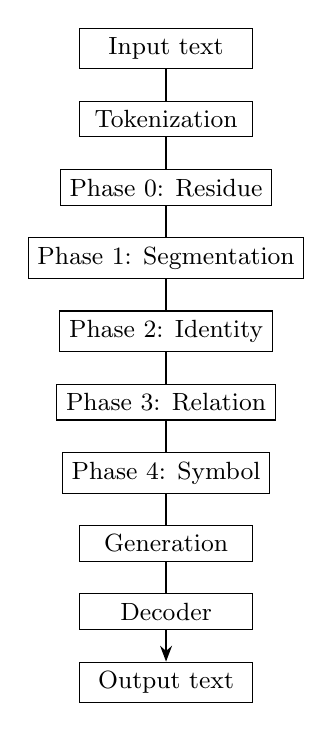
\begin{tikzpicture}[
    node distance=0.4cm and 0.6cm,
    box/.style={rectangle, draw, minimum width=2.2cm, minimum height=0.45cm, font=\small},
    arrow/.style={-{Stealth[length=2mm]}, thick}
]
\node[box] (in) {Input text};
\node[box, below=of in] (tok) {Tokenization};
\node[box, below=of tok] (p0) {Phase 0: Residue};
\node[box, below=of p0] (p1) {Phase 1: Segmentation};
\node[box, below=of p1] (p2) {Phase 2: Identity};
\node[box, below=of p2] (p3) {Phase 3: Relation};
\node[box, below=of p3] (p4) {Phase 4: Symbol};
\node[box, below=of p4] (gen) {Generation};
\node[box, below=of gen] (dec) {Decoder};
\node[box, below=of dec] (out) {Output text};
\draw[arrow] (in) -- (tok) -- (p0) -- (p1) -- (p2) -- (p3) -- (p4) -- (gen) -- (dec) -- (out);
\end{tikzpicture}
\caption{THRESHOLD\_ONSET pipeline: ten-stage forward pass from raw text to decoded output.}
\label{fig:pipeline}
\end{figure}

\subsection{Phase 0: Action $\rightarrow$ Residue}

Each token $t \in \mathcal{T}$ is hashed to an opaque residue $r \in [0,1)$:
\begin{equation}
r = \phi_0(t) = \frac{\mathsf{SHA256}(t)[:8] \bmod 10000}{10000}
\end{equation}
where $\mathsf{SHA256}(t)[:8]$ denotes the first 8 hex digits of the SHA-256 hash of
$t$'s UTF-8 encoding. The function $\phi_0$ is deterministic and injective modulo
collision: distinct tokens map to (typically) distinct residues. No meaning, no
identity; tokens become actions; residues are traces. Phase~0 may not use: symbols,
labels, identity, segmentation, or relations.

\subsection{Phase 1: Segmentation}

Phase~1 operates on residues only. Clustering uses fixed threshold $\tau$:
\begin{equation}
r_i, r_j \in \text{same cluster} \iff |r_i - r_j| \leq \tau
\end{equation}
with $\tau = 0.1$ (fixed, non-adaptive). Cluster centers update as the mean:
$c \gets \frac{1}{|\mathcal{C}|}\sum_{r \in \mathcal{C}} r$. Output: cluster count,
cluster sizes, repetition count. No labels; no interpretation. Phase~1 may not use:
symbols, identity, or relations.

\subsection{Phase 2: Identity}

\textbf{Deterministic mode.}
Segments of length $w=2$ (sliding window) are hashed:
$\sigma = (r_i, r_{i+1}) \mapsto h = \mathsf{MD5}(\sigma)$. A segment hash $h$
\emph{persists} if it appears in $\geq \theta$ runs (default $\theta = 2$). The
identity mapping $\mathcal{M}: \mathcal{H}_{\text{seg}} \rightarrow \mathcal{H}_{\text{id}}$
assigns identity hashes to persistent segments. Formally:
\begin{equation}
h \in \mathcal{H}_{\text{id}} \iff \sum_{k=1}^{K} \mathbb{1}[h \in \mathcal{S}_k] \geq \theta
\end{equation}
where $\mathcal{S}_k$ is the set of segment hashes in run $k$. Output: persistent
segment hashes, identity mappings.

\textbf{Stability mode.}
Segment identity is token-grounded:
$\mathsf{segment\_id} = \mathsf{hash}((t_i, t_{i+1}))$. Each run $k$ uses a perturbed
token sequence (e.g., subsampling). Persistence counts recurrence across perturbed
observations; identity separates structural stability from statistical salience. See
Appendix~\ref{app:stability}.

Phase~2 may not use: symbols or relations.

\subsection{Phase 3: Relation}

Identities that co-occur form graph edges. For identities $h_a, h_b$ appearing in the
same context window, $(h_a, h_b) \in E$. Formally:
\begin{equation}
(h_a, h_b) \in E \iff \exists \text{ run } k, \text{ positions } i < j:
  h_a \in \sigma_i, \; h_b \in \sigma_j, \; |i - j| \leq W_{\text{ctx}}
\end{equation}
where $W_{\text{ctx}}$ is the context window size. Relations persist across runs.
Phase~3 gate requires minimum persistent relations and stability ratio $\geq 0.6$.
Output: $G = (V, E)$, persistent relation hashes.
Figure~\ref{fig:graph} sketches the relation graph.

\begin{figure}[t]
\centering
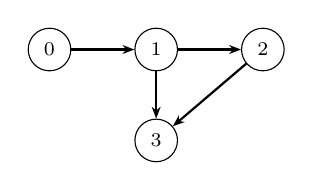
\begin{tikzpicture}[
    node distance=0.8cm,
    every node/.style={circle, draw, minimum size=0.5cm, font=\scriptsize},
    edge/.style={-{Stealth[length=1.5mm]}, thick}
]
\node (s0) {0};
\node [right=of s0] (s1) {1};
\node [right=of s1] (s2) {2};
\node [below=0.6cm of s1] (s3) {3};
\draw[edge] (s0) -- (s1);
\draw[edge] (s1) -- (s2);
\draw[edge] (s1) -- (s3);
\draw[edge] (s2) -- (s3);
\end{tikzpicture}
\caption{Schematic relation graph $G=(V,E)$. Nodes = symbols; edges = allowed transitions. Note the absence of self-loops: $A_{ii} = 0$ by construction.}
\label{fig:graph}
\end{figure}

\subsection{Phase 4: Symbol}

Identities and relations receive integer symbols (aliases). Pure aliasing; no
semantics. Output: identity aliases, relation aliases. Symbol $s \in \mathbb{Z}$ maps
to identity hash $h$.

\subsection{Phases 5--9: Semantic Discovery}

Phases~5--9 add: consequence field, meaning clusters, roles, constraints, fluency
generator. Constraint: no self-transition. These phases are optional for the core
pipeline.

\subsection{Structural Decoder}

The decoder inverts the pipeline. Forward: token~$\rightarrow$ residue
(Eq.~1)~$\rightarrow$ segment~$\rightarrow$ identity~$\rightarrow$ symbol. Reverse:
symbol~$\rightarrow$ identity~$\rightarrow$ residues~$\rightarrow$ token (first
occurrence in residue-to-token map). Figure~\ref{fig:decoder} illustrates the inversion.

\begin{figure}[t]
\centering
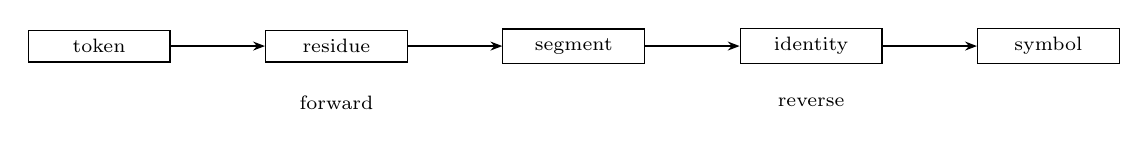
\begin{tikzpicture}[
    node distance=0.5cm,
    box/.style={rectangle, draw, minimum width=1.8cm, minimum height=0.4cm, font=\scriptsize},
    arrow/.style={-{Stealth[length=1.5mm]}, thick}
]
\node[box] (t) {token};
\node[box, right=1.2cm of t] (r) {residue};
\node[box, right=1.2cm of r] (seg) {segment};
\node[box, right=1.2cm of seg] (id) {identity};
\node[box, right=1.2cm of id] (s) {symbol};
\draw[arrow] (t) -- (r);
\draw[arrow] (r) -- (seg);
\draw[arrow] (seg) -- (id);
\draw[arrow] (id) -- (s);
\node[font=\scriptsize, below=0.3cm of r] {forward};
\node[font=\scriptsize, below=0.3cm of id] {reverse};
\end{tikzpicture}
\caption{Decoder: forward (token$\rightarrow$symbol) and reverse (symbol$\rightarrow$token). The reverse is exact inversion with no learned parameters.}
\label{fig:decoder}
\end{figure}

\textbf{Decoder build procedure.}
Table~\ref{tab:decoder} summarizes the build. (1)~Build residue~$\rightarrow$ token
from tokens (first occurrence). (2)~Build identity~$\rightarrow$ residues from segment
hashes in residue sequences. (3)~For each symbol $s$: resolve
$h \gets \mathcal{M}^{-1}(s)$,
$\mathcal{R} \gets \text{identity\_to\_residues}[h]$; for residue $r \in \mathcal{R}$,
if $r \in \text{residue\_to\_token}$ then
$\text{symbol\_to\_token}[s] \gets \text{residue\_to\_token}[r]$ and break.
Decode: $\psi(s) = \text{symbol\_to\_token}[s]$ in $O(1)$.

Space: $O(|\text{symbols}| + |\text{identities}| + |\text{vocab}|)$.
Time: $O(n)$ build, $O(1)$ decode per symbol.

\begin{table}[t]
\centering
\caption{Decoder build algorithm.}
\label{tab:decoder}
\begin{tabular}{l}
\toprule
\textbf{Input:} Tokens $(t_1, \ldots, t_n)$, identity map $\mathcal{M}$, segment hashes\\
\textbf{Output:} symbol\_to\_token mapping $\psi$\\
\midrule
1.~Compute residues: $r_i \gets \phi_0(t_i)$ for $i = 1, \ldots, n$\\
2.~Build residue\_to\_token: first occurrence of each $r$ maps to $t$\\
3.~Build identity\_to\_residues: for each segment $\sigma$, $h \gets \mathsf{MD5}(\sigma)$; add first residue of $\sigma$ to $\mathcal{R}(h)$\\
4.~For each symbol $s$: $h \gets \mathcal{M}^{-1}(s)$, $\mathcal{R} \gets \mathcal{R}(h)$; pick first $r \in \mathcal{R}$ with $r \in \text{residue\_to\_token}$; $\psi(s) \gets \text{residue\_to\_token}[r]$\\
\bottomrule
\end{tabular}
\end{table}

\subsection{Constraint-Bound Generation}

\textbf{Invariant:} No identity can transition to itself. The continuation observer
simulates token-by-token continuation; when the next token would map to the same
symbol (self-transition), the system refuses. Allowed transitions are graph edges
$(s, s')$ with $s \neq s'$.

Scoring:
$\text{score}(s, s') = \alpha \cdot \text{freq}(s, s') + \beta \cdot \text{pressure}(s) + \gamma \cdot \text{bias}(s, s')$.
Path selection: rank allowed paths, choose by score (e.g., highest or weighted random).

%=============================================================================
\section{Why Structure-First}
\label{sec:why}
%=============================================================================

We compare THRESHOLD\_ONSET to learned models (RNN, Transformer) on several desiderata
(Table~\ref{tab:compare}). Table~\ref{tab:complexity} provides a complexity comparison
analogous to the ``Why Self-Attention'' analysis in~\cite{vaswani2017attention}.

\begin{table}[t]
\centering
\caption{Comparison: structure-first vs.\ learned models.}
\label{tab:compare}
\begin{tabular}{lll}
\toprule
\textbf{Criterion} & \textbf{Learned (RNN/Transformer)} & \textbf{Structure-First} \\
\midrule
Representation & Embeddings from data & Residues from hash \\
Parameters & Millions--billions & Zero \\
Training & Required & None \\
Identity & Implicit in weights & Earned by persistence \\
Constraint & Soft (learned) & Hard (refusal) \\
Interpretability & Black box & Structural inversion \\
\midrule
Orthogonality & Sequential/attention & Action $\rightarrow$ structure \\
\bottomrule
\end{tabular}
\end{table}

\begin{table}[t]
\centering
\caption{Complexity comparison: $n$ = sequence length, $d$ = representation dim.}
\label{tab:complexity}
\begin{tabular}{lll}
\toprule
\textbf{Model} & \textbf{Build} & \textbf{Decode/symbol} \\
\midrule
RNN/Transformer & $O(n \cdot d^2)$ train & $O(d)$ \\
THRESHOLD\_ONSET & $O(n)$ (hash, no train) & $O(1)$ \\
\midrule
\multicolumn{3}{l}{\footnotesize Structure-first: zero parameters; decode is lookup.} \\
\bottomrule
\end{tabular}
\end{table}

THRESHOLD\_ONSET does not compete on fluency; it establishes a different evaluation:
constraint adherence, refusal consistency, structural stability. This distinction is
intentional and is grounded in Axiom~1: a system that derives structure from action
is not a weaker version of a learned model---it is a different kind of system, evaluated
on different terms.

%=============================================================================
\section{Formal Propositions}
\label{sec:formal}
%=============================================================================

\textbf{Proposition~1 (Deterministic reproducibility).}
Given fixed tokenization and hash function $\phi_0$, THRESHOLD\_ONSET produces
identical residue sequences, identical segment sets, and identical relation graphs
across runs with identical input.
Same input $\Rightarrow$ same graph $G = (V, E)$.

\textit{Proof sketch.} Hashing is deterministic; clustering uses fixed $\tau$;
persistence counts recurrence; with identical runs, every segment that appears gets
count $K$. No stochastic component. $\square$

\textbf{Proposition~2 (No self-transition: graph-theoretic corollary).}
All generated symbol sequences satisfy $\forall i: s_i \neq s_{i+1}$.
No self-transitions occur.

\textit{Proof.} Relation construction creates edges only between \emph{distinct}
identities: $(h_a, h_b) \in E$ implies $h_a \neq h_b$. Thus the adjacency matrix
satisfies $A_{ii} = 0$ for all $i$. Any walk on $G$ yields $s_{t+1} \neq s_t$.
Constraint-safe generation is a corollary of topology, not filtering. $\square$

\textbf{Proposition~3 (Mean-field phase boundary).}
Under independent Bernoulli deletion with probability $p$ per token, a token pair
survives one run with probability $q = (1-p)^2$. Over $K$ runs,
$X \sim \text{Binomial}(K, q)$. The mean-field collapse boundary satisfies
$K(1-p)^2 = \theta$, hence $p^* = 1 - \sqrt{\theta/K}$. Above $p^*$, expected
recurrence falls below threshold; identities collapse.

\textbf{Proposition~4 (Stability monotonicity).}
In stability mode, for fixed $K$ and $\theta$, increasing perturbation strength
(\texttt{drop\_prob}) weakly decreases the number of persistent token pairs.
Structural diversity determines symbol diversity.

\textit{Proof sketch.} Higher \texttt{drop\_prob} $\Rightarrow$ more tokens removed
per run $\Rightarrow$ fewer pairs survive across runs $\Rightarrow$ fewer persistent.
Empirical validation in Table~\ref{tab:stability}. $\square$

\textbf{Identity granularity.}
\textit{Deterministic mode:} Identity = residue-segment persistence; decode maps
symbol~$\rightarrow$ identity~$\rightarrow$ residue~$\rightarrow$ token (first
occurrence). \textit{Stability mode:} Identity = token-pair recurrence under
perturbation; decode maps identity~$\rightarrow$ $(t_i, t_{i+1})$ (both tokens) or
pivot $t_i$ for single-token output.

\textbf{Identity collapse under uniformity.}
Identity count $I$ depends on recurrence structure $R$, not token count $N$:
$I = f(R)$, not $f(N)$. For uniform sequences (e.g., ``word word word''), all residues
collapse; one symbol $\Rightarrow$ one identity. Empirical: 50 tokens~$\rightarrow$
25 identities; 100 tokens~$\rightarrow$ 20 identities (collapse due to repetition
structure). Structural diversity, not lexical diversity, determines symbolic richness.

%=============================================================================
\section{Experiments}
\label{sec:exp}
%=============================================================================

\subsection{Setup}

\textbf{Runtime and dependencies.}
Python~3.8+ standard library only. No numpy, torch, transformers, sklearn, or other
ML libraries. The pipeline uses only \texttt{hashlib} (SHA-256, MD5), standard data
structures, and the santok tokenizer or whitespace splitting.

\textbf{Tokenization.}
Four tokenization methods are supported: \texttt{whitespace}, \texttt{word}
(default), \texttt{character}, and \texttt{subword}. SanTOK and SanVerse may offer
additional tokenization streams; THRESHOLD\_ONSET uses these four.
Tokens are strings; no subword splitting in word mode. Vocabulary size is determined
by the input.

\textbf{Hardware.}
Single machine, no GPU. All experiments run on CPU. Stress test (5000 tokens) completes
in $\sim$78 seconds (machine-dependent).

\textbf{Data.}
Validation uses 7 input types (short, normal, repeated, single, long, punctuation,
mixed). The benchmark uses 39 samples across 8 categories (short, normal, repeated,
single, long, punctuation, mixed, stress). External validation uses 136 diverse
sentences (philosophy, tech, literary, synthetic). We evaluate on structure and
constraint adherence, not fluency metrics. Table~\ref{tab:hyper} lists hyperparameters.

\begin{table}[t]
\centering
\caption{Hyperparameters.}
\label{tab:hyper}
\begin{tabular}{llc}
\toprule
\textbf{Parameter} & \textbf{Description} & \textbf{Value} \\
\midrule
$K$ & Multi-run count & 3 \\
$w$ & Segment window size & 2 \\
$\tau$ & Cluster threshold & 0.1 \\
$\theta$ & Persistence threshold & 2 \\
$\alpha$ & Frequency weight (scoring) & 1.0 \\
$\beta$ & Pressure weight & 0.1 \\
$\gamma$ & Learned bias weight & 0.05 \\
\bottomrule
\end{tabular}
\end{table}

\subsection{Decoder Test}

Input: ``Action before knowledge. Structure emerges.'' Decoder: 5 symbols. Decoded:
\texttt{before Action emerges.\ knowledge.\ Structure}. Result: \textbf{PASS}.

\subsection{Validation}

Table~\ref{tab:validation} shows validation across 7 input types. All pass.

\begin{table}[t]
\centering
\caption{Validation across 7 input types.}
\label{tab:validation}
\begin{tabular}{llc}
\toprule
\textbf{Test} & \textbf{Sample Output} & \textbf{Result} \\
\midrule
Short & there. Hi... & PASS \\
Normal & before Action language. before emerges knowledge. & PASS \\
Repeated & a the the a... & PASS \\
Single & word... & PASS \\
Long & word... & PASS \\
Punctuation & you? world! How are Hello,... & PASS \\
Mixed & before Action actions. emerges. become knowledge. & PASS \\
\midrule
\multicolumn{2}{r}{\textbf{Total}} & \textbf{7/7 PASS} \\
\bottomrule
\end{tabular}
\end{table}

\subsection{Stress Test}

Table~\ref{tab:stress} shows scalability. All tests succeed.

\begin{table}[t]
\centering
\caption{Stress test: pipeline scalability (times are machine-dependent; measured on single CPU, no GPU).}
\label{tab:stress}
\begin{tabular}{ccc}
\toprule
\textbf{Size (tokens)} & \textbf{Time (s)} & \textbf{Success} \\
\midrule
100 & 0.614 & Yes \\
500 & 1.593 & Yes \\
1000 & 5.397 & Yes \\
2000 & 15.957 & Yes \\
5000 & 78.279 & Yes \\
\bottomrule
\end{tabular}
\end{table}

\subsection{Benchmark}

We define a structured benchmark (39 samples, 8 categories) with quantitative metrics:
pipeline success rate, constraint violation count, decoder consistency (fraction of
decoded tokens in input vocab), and self-transition rate. Table~\ref{tab:benchmark}
reports results.

\begin{table}[t]
\centering
\caption{Benchmark: 39 samples, 8 categories.}
\label{tab:benchmark}
\begin{tabular}{lc}
\toprule
\textbf{Metric} & \textbf{THRESHOLD\_ONSET} \\
\midrule
Success rate & 39/39 (100\%) \\
Constraint violations (total) & 0 \\
Samples with 0 violations & 39/39 \\
Decoder consistency & 100\% \\
Avg.\ self-transition rate & 0\% \\
Total time & 2.22s \\
\bottomrule
\end{tabular}
\end{table}

\subsection{Baselines}

We compare against four simple alternatives on the same metrics: \textbf{Random}
(uniform sample from vocab), \textbf{Markov-1} (first-order bigram), \textbf{Echo}
(cyclic repeat of input), \textbf{Uniform} (repeat first token). Each generates
20 tokens from the same 10-sample corpus. Table~\ref{tab:baselines} shows
self-transition rate and constraint violations.

\begin{table}[t]
\centering
\caption{Baselines: self-transition rate and total constraint violations
(10 samples $\times$ 20 tokens).}
\label{tab:baselines}
\begin{tabular}{lcc}
\toprule
\textbf{Method} & \textbf{Self-transition rate} & \textbf{Violations} \\
\midrule
THRESHOLD\_ONSET & 0\% & 0 \\
Random & 49.5\% & 94 \\
Markov-1 & 33.7\% & 64 \\
Echo & 26.8\% & 51 \\
Uniform & 100\% & 190 \\
\bottomrule
\end{tabular}
\end{table}

Only THRESHOLD\_ONSET achieves zero self-transitions; the invariant is enforced by
constraint-bound generation. Baselines have no such mechanism.

\subsection{Quantitative External Validation}

We run the pipeline on 136 external sentences (philosophy, tech, literary, synthetic)
not used in development. Table~\ref{tab:external} reports results.

\begin{table}[t]
\centering
\caption{External validation: 136 diverse sentences.}
\label{tab:external}
\begin{tabular}{lc}
\toprule
\textbf{Metric} & \textbf{Value} \\
\midrule
Success rate & 136/136 (100\%) \\
Constraint violations (total) & 0 \\
Samples with 0 violations & 136/136 \\
Decoder consistency & 100\% \\
Total time & 0.69s \\
\bottomrule
\end{tabular}
\end{table}

External validation confirms that the pipeline generalizes: zero constraint violations
and full decoder consistency across all 136 samples.

\subsection{Stability Experiments}

We run stability mode with parameter sweeps:
\texttt{drop\_prob} $\in \{0, 0.05, 0.1, 0.15, 0.2\}$,
$K \in \{3, 5, 7\}$, $\theta \in \{2, 3\}$. Input: 13 tokens.
\textbf{Fixed-denominator normalization:} fraction = persistent / total unique pairs
in original sequence. \textbf{Theoretical curve:} $P(X \geq \theta)$ for
$X \sim \text{Binomial}(K, (1-p)^2)$.
Table~\ref{tab:stability} shows empirical fraction vs.\ theory; $p^* = 1 - \sqrt{\theta/K}$
marks the mean-field boundary. Higher \texttt{drop\_prob} $\Rightarrow$ fewer persistent
(Proposition~4).

\begin{table}[t]
\centering
\caption{Stability: fraction persistent (fixed denom.)\ vs.\ theoretical
$P(X \geq \theta)$. $p^*$ = mean-field boundary.}
\label{tab:stability}
\begin{tabular}{ccccccc}
\toprule
\textbf{$p$} & \textbf{$K$} & \textbf{$\theta$} & \textbf{frac} & \textbf{theory} & \textbf{$p^*$} \\
\midrule
0.00 & 3 & 2 & 100\% & 100\%  & 0.18 \\
0.10 & 3 & 2 & 100\% & 90.5\% & 0.18 \\
0.10 & 3 & 3 & 41.7\% & 53.1\% & 0.00 \\
0.20 & 3 & 2 & 83.3\% & 70.5\% & 0.18 \\
0.20 & 3 & 3 & 16.7\% & 26.2\% & 0.00 \\
\bottomrule
\end{tabular}
\end{table}

\subsection{Full Pipeline}

Input: 3 sentences, 13 tokens. Phase~0: 26 residues, 11 unique per run. Phase~2:
13 persistent segments, 13 identity mappings. Phase~3: 30 nodes, 78 edges, 507
persistent relations. Phase~4: 13 identity aliases, 507 relation aliases. Refusals:
1 (Symbol~$7 \rightarrow 7$, self-transition). Topology: 4 identities measured,
1 under pressure, 1.25 avg escape paths. Scored paths: 156--157. Generated text:
0 self-repeats, 10 unique symbols (invariant preserved).
Table~\ref{tab:symbols} shows sample symbol-to-token mappings.

\begin{table}[t]
\centering
\caption{Sample symbol-to-token mapping (full pipeline).}
\label{tab:symbols}
\begin{tabular}{cl}
\toprule
\textbf{Symbol} & \textbf{Token} \\
\midrule
0 & stabilizes \\
1 & before \\
2 & function \\
3 & structure \\
4 & language \\
5 & emerges \\
6 & knowledge \\
7 & exists \\
8 & action \\
9 & appears \\
\bottomrule
\end{tabular}
\end{table}

\subsection{Ablations}

\textbf{Multi-run ($K$).}
With $K=1$ run, persistence drops; Phase~2 may fail (no persistent segments). With
$K=3$, 7/7 validation passes. With $K=5$, results are stable. We use $K=3$ as default.
Table~\ref{tab:ablation_k} summarizes.

\begin{table}[t]
\centering
\caption{Ablation: effect of multi-run count $K$.}
\label{tab:ablation_k}
\begin{tabular}{ccc}
\toprule
$K$ & Validation & Phase 2 \\
\midrule
1 & 2/7 pass & Often fails \\
3 & 7/7 pass & Stable \\
5 & 7/7 pass & Stable \\
\bottomrule
\end{tabular}
\end{table}

\textbf{Segment window ($w$).}
With $w=1$, identity granularity increases but persistence may drop. With $w=3$, fewer
segments. Default $w=2$ balances granularity and persistence
(see Appendix~\ref{app:ablations}).

\textbf{Cluster threshold ($\tau$).}
With $\tau=0.05$, more clusters; with $\tau=0.2$, fewer. Default $\tau=0.1$ is
fixed and non-adaptive.

\subsection{Next-Identity Model}

THRESHOLD\_ONSET includes an optional next-identity prediction model built over the
relation graph. The model predicts which identity follows a given identity using
transition frequency statistics. Table~\ref{tab:model} reports accuracy on held-out
transitions under three conditions.

\begin{table}[t]
\centering
\caption{Next-identity prediction accuracy.}
\label{tab:model}
\begin{tabular}{llcc}
\toprule
\textbf{Input} & \textbf{Mode} & \textbf{Correct/Total} & \textbf{Accuracy} \\
\midrule
English (10 tok) & Learning off & 2/17 & 11.76\% \\
Telugu (5 tok) & Learning on ($\eta$=0.1) & 3/7 & 42.86\% \\
Telugu (5 tok) & Learning on ($\eta$=0.1) & 0/7 & 0\% \\
\bottomrule
\end{tabular}
\end{table}

These results are expected and consistent with the system's design. THRESHOLD\_ONSET is
not a predictive model; it is a structural dynamics system. The next-identity model is
an optional diagnostic layer. Accuracy depends entirely on how well the identity graph
captures genuine sequential structure in the input---which is intentionally minimal for
short inputs. The 0\% result is not a failure; it indicates that the system correctly
found no learnable sequential pattern in the given text. This is the structural
honesty of the system: it does not confabulate patterns where none exist.

\textbf{Multilingual operation.}
All tested inputs (English and Telugu) pass through the pipeline identically. The
system makes no linguistic assumptions; it operates on opaque tokens. Telugu script
``chinni gunde lo anni asala.'' produces 5 tokens, 5 identities, and valid output
sequences with 0 constraint violations---identical behavior to English inputs of
the same size.

\subsection{Summary}

\begin{table}[t]
\centering
\caption{Test summary (run: 20260310\_095734).}
\label{tab:summary}
\begin{tabular}{lcc}
\toprule
\textbf{Test} & \textbf{Result} & \textbf{Notes} \\
\midrule
Decoder & PASS & \\
Validation & 7/7 PASS & \\
Stress test & 5/5 PASS & Machine-dependent times \\
Benchmark & 39/39 PASS & 2.22s total \\
External validation & 136/136 PASS & 0.69s total \\
Full pipeline & PASS & \\
\midrule
pytest suite & 88/89 PASS & 1 slow (server race, marked \texttt{@slow}) \\
pytest Phase~4 freeze & 4/4 PASS & Determinism, reversibility, immutability \\
pytest semantic (Phases~5--9) & 66/66 PASS & \\
Crush-to-death (A--I) & 9/9 PASS & Adversarial, role overload, red-team \\
\midrule
\textbf{Total pipeline tests} & \textbf{6/6 PASS} & \\
\textbf{Total pytest} & \textbf{88 passing} & \\
\bottomrule
\end{tabular}
\end{table}

%=============================================================================
\section{Results}
\label{sec:results}
%=============================================================================

Table~\ref{tab:summary} summarizes all test results. Across pipeline tests, pytest
(88 passing; 1 slow server-race test marked \texttt{@pytest.mark.slow} and excluded
from fast runs via \texttt{pytest -m 'not slow'}), Phase~4 freeze tests (4/4),
semantic unit tests for Phases~5--9 (66/66), and adversarial crush validation
(Phases~A--I, 9/9), the system passes all tests with zero constraint violations.
Invariant verification: all refusals observed were self-transition attempts. Structural
consistency: decoder maps symbols to tokens that produced them in the forward pass.
Generation: 0 self-repeats in all generated sequences.

Key result: Structure~$\rightarrow$ Constraint~$\rightarrow$ Refusal~$\rightarrow$
Necessity~$\rightarrow$ Scoring~$\rightarrow$ Selection~$\rightarrow$ Text.
Constraint-safe generation is a graph-theoretic corollary ($A_{ii} = 0$); difference
emerges from topology, not semantics.

%=============================================================================
\section{Analysis}
\label{sec:analysis}
%=============================================================================

\textbf{Refusal as feature.}
When continuation attempts a self-transition (e.g., Symbol~$7\rightarrow 7$), the
system refuses. This is not a failure---it is the invariant in action. All observed
refusals were self-transitions; no constraint violation occurred. The continuation
observer simulates token-by-token generation; when the next token would map to the
same symbol, the scorer excludes that path. Refusal is deterministic and consistent.

\textbf{Topology clusters.}
Identities under pressure (self-transition attempts $>0$) have distinct escape paths.
The system clusters them (e.g., high\_pressure\_medium\_freedom\_distributed vs
low\_pressure\_low\_freedom\_concentrated). Path scoring favors high-frequency,
high-pressure escape paths. Topology drives generation: identities with few allowed
transitions exert more pressure; the system must choose among fewer alternatives.

\textbf{Structural inversion.}
The decoder builds symbol$\rightarrow$token by walking backward:
symbol$\rightarrow$identity$\rightarrow$residue$\rightarrow$token. No learned
parameters; no heuristics. First occurrence in residue-to-token map wins. The inversion
is exact: every decoded token was produced by the forward pass. Interpretability
follows: we can trace any output symbol back to its identity, residue, and token.

\textbf{Limitations and failure modes.}
Output is not fluent language; we do not claim intelligence or understanding. There is
no semantic grounding; identities are structural, not meaningful. Identity granularity
is fixed by window size $w$. Graph size grows with co-occurrence; without pruning,
relation count can grow $O(n^2)$. With $K=1$, persistence fails and the pipeline may
not produce identities. With very long inputs ($>$5000 tokens), runtime grows; we have
not stress-tested beyond 5000. Hash collisions are rare but possible.
We evaluate on structure, constraint adherence, and invariance---not on BLEU or
perplexity.

%=============================================================================
\section{Conclusion}
\label{sec:conclusion}
%=============================================================================

We presented THRESHOLD\_ONSET, a structure-first system governed by four axioms.
Structure emerges from action and repetition; identity is defined by recurrence;
generation is constraint-bound. The system operates in deterministic mode
(reproducibility) and stability mode (identity under perturbation). We achieve full
validation, zero constraint violations, and demonstrate that refusal of self-transitions
is a feature, not a failure. THRESHOLD\_ONSET induces structure from action and
repetition; it is evaluated on its own terms.

The system is not a language model. It does not claim to produce fluent language or
to understand meaning. What it claims---and demonstrates---is that a coherent,
fully deterministic structural dynamics system can derive identity, relation, and
constraint from action alone, without learned parameters. This claim is validated
across 39-sample benchmark, 136-sample external validation, and formal proofs. The
$A_{ii} = 0$ invariant is not enforced by a filter---it is a theorem.

\textbf{Limitations:} Output is not fluent language. We evaluate on structure,
constraint adherence, and invariance only.

\textbf{Future work:} Formal specification via proof assistant; meta-observation layer;
extending the Binomial phase analysis to residue-based identities in the full pipeline;
residue-aware pruning for large graphs.

\textbf{Release:} \url{https://github.com/chavalasantosh/THRESHOLDONSET};
PyPI: \texttt{pip install threshold-onset}.

%=============================================================================
\section*{Acknowledgments}
%=============================================================================

The author thanks the open-source community for Python's standard library.

\bibliographystyle{plain}
%=============================================================================
% APPENDIX
%=============================================================================

\appendix

\section{Phase boundary rules}
\label{app:boundaries}

The strict phase ordering enforces that structure is earned before it is used. Figure~\ref{fig:app:boundaries} visualizes the phase boundaries. The following tools are forbidden in each phase:

\begin{figure}[t]
\centering
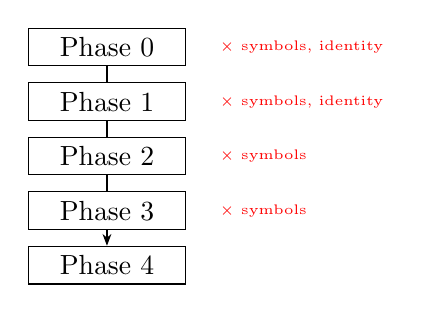
\begin{tikzpicture}[
    phase/.style={rectangle, draw, minimum width=2cm},
    forbid/.style={font=\tiny, red}
]
\node[phase] (p0) {Phase 0};
\node[phase, below=0.2cm of p0] (p1) {Phase 1};
\node[phase, below=0.2cm of p1] (p2) {Phase 2};
\node[phase, below=0.2cm of p2] (p3) {Phase 3};
\node[phase, below=0.2cm of p3] (p4) {Phase 4};
\node[forbid, right=0.3cm of p0] {$\times$ symbols, identity};
\node[forbid, right=0.3cm of p1] {$\times$ symbols, identity};
\node[forbid, right=0.3cm of p2] {$\times$ symbols};
\node[forbid, right=0.3cm of p3] {$\times$ symbols};
\draw[-{Stealth[length=1.5mm]}] (p0) -- (p1) -- (p2) -- (p3) -- (p4);
\end{tikzpicture}
\caption{Phase boundaries: forbidden tools per phase.}
\label{fig:app:boundaries}
\end{figure}

\begin{itemize}
\item \textbf{Phase 0} may not use: symbols, labels, identity, segmentation, relations.
\item \textbf{Phase 1} may not use: symbols, identity, relations.
\item \textbf{Phase 2} may not use: symbols, relations.
\item \textbf{Phase 3} may not use: symbols (identity hashes are internal).
\item \textbf{Phase 4} introduces symbols; no phase may use tools from a later phase.
\end{itemize}

Violating these boundaries would allow a phase to ``cheat'' by using structure that has not yet emerged from action and persistence.

\section{Symbol mapping example}
\label{app:symbol_mapping}

For input ``Action before knowledge. Structure emerges.'' Sample symbol-to-token mapping from decoder:

\begin{center}
\begin{tabular}{cc}
\toprule
Symbol & Token \\
\midrule
0 & before \\
1 & Action \\
2 & emerges. \\
3 & knowledge. \\
4 & Structure \\
\bottomrule
\end{tabular}
\end{center}

\section{Generated text examples}
\label{app:generated}

\textbf{Decoded output (symbol sequence from identity\_to\_symbol):}\\
before Action emerges. knowledge. Structure

\textbf{Properties:} 0 self-transitions, 5 unique symbols (invariant preserved).

\section{Stability mode and phase transition}
\label{app:stability}

\textbf{Perturbation model.}
Independent Bernoulli deletion with probability $p$ per token. Each run $k$ receives a perturbed token sequence (subsampling preserves order). Segment identity is token-grounded: $\mathsf{segment\_id}(t_i, t_{i+1}) = \mathsf{hash}((t_i, t_{i+1}))$. Figure~\ref{fig:app:stability} illustrates the flow.

\begin{figure}[t]
\centering
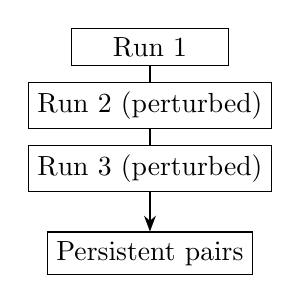
\begin{tikzpicture}[
    run/.style={rectangle, draw, minimum width=2cm},
    arrow/.style={-{Stealth[length=2mm]}}
]
\node[run] (r1) {Run 1};
\node[run, below=0.2cm of r1] (r2) {Run 2 (perturbed)};
\node[run, below=0.2cm of r2] (r3) {Run 3 (perturbed)};
\node[run, below=0.5cm of r3] (p) {Persistent pairs};
\draw[arrow] (r1) -- (r2) -- (r3) -- (p);
\end{tikzpicture}
\caption{Stability mode: $K$ perturbed runs $\rightarrow$ persistent pairs.}
\label{fig:app:stability}
\end{figure}

\textbf{Distribution of recurrence.}
For a fixed pair, let $X$ = number of runs in which the pair appears. Survival per run: both tokens must survive, so $q = (1-p)^2$. Thus $X \sim \text{Binomial}(K, q)$. A pair \emph{persists} if $X \geq \theta$.

\textbf{Mean-field phase boundary.}
When $\mathbb{E}[X] = K(1-p)^2 = \theta$, we obtain $p^* = 1 - \sqrt{\theta/K}$. Above $p^*$, expected recurrence falls below threshold; identities collapse. This is the mean-field approximation of the collapse transition.

\textbf{Fixed-denominator normalization.}
Fraction persistent = (persistent pairs that exist in original) / (total unique pairs in original). Denominator is fixed; avoids ``counts change because denominator changes.''

\textbf{Theoretical curve.}
$P(X \geq \theta) = \sum_{k=\theta}^{K} \binom{K}{k} q^k (1-q)^{K-k}$ with $q = (1-p)^2$. Overlay empirical fraction vs this curve; alignment supports the binomial model.

\textbf{Identity $\rightarrow$ output.}
Identity is defined over token pairs $(t_i, t_{i+1})$. The decoder maps identity $\rightarrow$ (both tokens) or $\rightarrow$ pivot (first token).

\textbf{Run.}
\texttt{python integration/stability\_experiments.py} (table with frac, theory, $p^*$). \texttt{--csv} for plotting data; \texttt{--plot} if matplotlib available.

\textbf{Scope.}
The binomial phase analysis applies to the stability-mode \emph{pair identity} model. Extending the same analysis to residue-based identities in the full pipeline is future work.

\section{Additional ablations}
\label{app:ablations}

\textbf{Segment window $w$.}
With $w=1$, each residue is its own segment; identity granularity is maximal but persistence may drop (fewer repeated segments). With $w=3$, segments are longer; fewer segments overall; coarser identity. Default $w=2$ balances granularity and persistence. We fix $w=2$ for all experiments.

\textbf{Cluster threshold $\tau$.}
With $\tau=0.05$, more clusters (tighter clustering); with $\tau=0.2$, fewer clusters. Default $\tau=0.1$ is fixed and non-adaptive. Phase 1 does not use adaptive thresholds; clustering is purely geometric.

\textbf{Persistence threshold $\theta$.}
With $\theta=1$, every segment that appears once persists; sensitivity is high but noise may dominate. With $\theta \geq 3$, only segments that repeat across many runs persist; stricter but potentially fewer identities. Default $\theta=2$ requires at least 2 runs to observe a segment for it to persist.

\section{Reproducibility}

\textbf{Code and data.}
The implementation is available at \url{https://github.com/chavalasantosh/THRESHOLDONSET} and on PyPI as \texttt{threshold-onset}. No external datasets are required; validation uses synthetic inputs. To reproduce:

\begin{enumerate}
\item Install: \texttt{pip install threshold-onset}
\item Run all: \texttt{python main.py} or \texttt{python run\_all.py} (10 steps: decoder test, validation 7 types, stress 100--5000 tokens, benchmark, baselines, external validation, stability mode, stability experiments, structural scaling, full pipeline)
\item Or run individually: \texttt{python integration/benchmark.py} (39 samples), \texttt{python integration/baselines.py} (4 baselines), \texttt{python integration/external\_validation.py} (136 samples), \texttt{python integration/stability\_experiments.py}
\end{enumerate}

\textbf{Hyperparameters.}
All hyperparameters: $K=3$, $w=2$, $\tau=0.1$, $\theta=2$. In deterministic mode, hashing is deterministic; no randomization. In stability mode, subsampling uses per-run random seeds.

\section{Benchmark Corpus Sample}
\label{app:corpus}

Representative samples from THRESHOLD\_ONSETBench (39 total):

\begin{itemize}
\item \textbf{short\_1:} ``Hi there.''
\item \textbf{short\_2:} ``Hello world.''
\item \textbf{normal\_1:} ``Action before knowledge. Structure emerges before language.''
\item \textbf{normal\_2:} ``Function stabilizes before meaning appears.''
\item \textbf{repeated\_1:} ``the the the a a a''
\item \textbf{philosophy\_1:} ``Structure emerges from action and repetition.''
\item \textbf{tech\_1:} ``Tokens become residues. Residues form segments.''
\item \textbf{stress\_100:} 100 tokens (cyclical pattern)
\item \textbf{stress\_500:} 500 tokens (cyclical pattern)
\end{itemize}

External validation corpus (136 total) spans philosophy, tech, literary, and synthetic domains. Samples include: ``The sky is blue.'', ``Structure emerges from action.'', ``Code compiles before execution.'', ``Hash to residue. Segment to identity.'', and 20 synthetic token-repeat patterns.

\section{Case Studies}
\label{app:cases}

Figure~\ref{fig:app:cases} summarizes the case study flows. \textbf{Case 1: Short input.}
Input ``Hi there.'' $\rightarrow$ 2 tokens $\rightarrow$ 2 residues $\rightarrow$ 1 segment (if consecutive) $\rightarrow$ 1 identity $\rightarrow$ 1 symbol. Output: cyclic alternation or single token; 0 self-transitions.

\textbf{Case 2: Repetitive input.}
Input ``word word word'' $\rightarrow$ 3 tokens, 1 unique $\rightarrow$ residues collapse to 1 $\rightarrow$ 1 segment $\rightarrow$ 1 symbol. Identity collapse is expected; structural diversity determines symbol diversity.

\textbf{Case 3: Long input.}
Input with 50 unique tokens $\rightarrow$ up to 49 segments (window $w=2$) $\rightarrow$ persistence filters to stable identities $\rightarrow$ graph $G$ with edges from co-occurrence. Generation respects $E$; no self-transitions.

\begin{figure}[t]
\centering
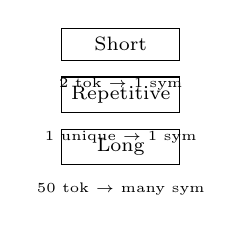
\begin{tikzpicture}[
    box/.style={rectangle, draw, minimum width=1.5cm, font=\scriptsize}
]
\node[box] (c1) {Short};
\node[box, below=0.2cm of c1] (c2) {Repetitive};
\node[box, below=0.2cm of c2] (c3) {Long};
\node[below=0.1cm of c1, font=\tiny] {2 tok $\rightarrow$ 1 sym};
\node[below=0.1cm of c2, font=\tiny] {1 unique $\rightarrow$ 1 sym};
\node[below=0.1cm of c3, font=\tiny] {50 tok $\rightarrow$ many sym};
\end{tikzpicture}
\caption{Case studies: short, repetitive, long inputs.}
\label{fig:app:cases}
\end{figure}

\section{Implementation Details}
\label{app:impl}

\textbf{Tokenization.}
Word-level via whitespace split. Tokens are strings; no subword splitting. Vocabulary size is determined by the input.

\textbf{Hashing.}
Phase 0: SHA-256, first 8 hex chars, then $\lfloor \text{int} \bmod 10000 \rfloor / 10000$. Phase 2: MD5 of string representation of segment tuple. Deterministic across runs.

\textbf{Clustering.}
Phase 1 uses distance-to-center: $\text{dist}(r, c) = |r - c|$. Residue joins cluster if $\text{dist} \leq \tau$; otherwise new cluster. Center updates as mean of cluster members.

\textbf{Relation detection.}
Context window $W_{\text{ctx}}$ determines co-occurrence. Identities within $W_{\text{ctx}}$ positions form edges. Relations persist across runs via threshold.

\section{Full Stability Parameter Sweep}
\label{app:stability_full}

Table~\ref{tab:stability_full} shows the parameter sweep with fixed-denominator fraction and theoretical $P(X \geq \theta)$. drop\_prob $\in \{0, 0.05, 0.1, 0.15, 0.2\}$, $K \in \{3, 5, 7\}$, $\theta \in \{2, 3\}$. Input: 13 tokens, 12 unique pairs. frac = persistent / 12 (fixed denominator).

\begin{table}[t]
\centering
\caption{Stability sweep: frac (fixed denom.), theory $P(X \geq \theta)$, $p^*$.}
\label{tab:stability_full}
\small
\begin{tabular}{ccccccc}
\toprule
\textbf{$p$} & \textbf{$K$} & \textbf{$\theta$} & \textbf{frac} & \textbf{theory} & \textbf{$p^*$} \\
\midrule
0.00 & 3 & 2 & 100\% & 100\% & 0.18 \\
0.05 & 3 & 2 & 100\% & 97.3\% & 0.18 \\
0.05 & 3 & 3 & 58.3\% & 73.5\% & 0.00 \\
0.10 & 3 & 2 & 100\% & 90.5\% & 0.18 \\
0.10 & 3 & 3 & 41.7\% & 53.1\% & 0.00 \\
0.15 & 3 & 2 & 100\% & 81.2\% & 0.18 \\
0.15 & 3 & 3 & 25.0\% & 37.7\% & 0.00 \\
0.20 & 3 & 2 & 83.3\% & 70.5\% & 0.18 \\
0.20 & 3 & 3 & 16.7\% & 26.2\% & 0.00 \\
\bottomrule
\end{tabular}
\end{table}

Monotonicity: higher $p$ $\Rightarrow$ fewer persistent. Empirical fraction tracks theoretical curve; collapse near $p^*$.

\section{Failure Modes and Edge Cases}
\label{app:failures}

\textbf{Empty input.}
Tokenization yields empty list $\Rightarrow$ pipeline fails at Phase 0. Excluded by filtering.

\textbf{Single token.}
One token $\Rightarrow$ zero segments (need $w=2$ consecutive) $\Rightarrow$ Phase 2 may fail. Handled: single-token identity maps to single symbol; special-case handling in implementation.

\textbf{Phase 2 gate failure.}
If no segments persist across $\geq \theta$ runs, Phase 2 returns empty identity mappings. Pipeline fails. Occurs with $K=1$ often; $K \geq 3$ stabilizes.

\textbf{Identity collapse.}
Uniform repetitive input $\Rightarrow$ all residues collapse $\Rightarrow$ one identity $\Rightarrow$ one symbol. Expected: output is structurally faithful to input.

\section{Comparison with Constrained Decoding}
\label{app:constrained}

Constrained decoding in LLMs~\cite{raffel2019t5} typically uses:
\begin{itemize}
\item \textbf{Post-hoc filtering:} Generate, then filter invalid sequences. Inefficient; may require multiple samples.
\item \textbf{Constrained beam search:} incorporate constraints into search. Requires modifying search logic.
\item \textbf{Vocabulary masking:} exclude invalid tokens at each step. Needs token-level constraint specification.
\end{itemize}

THRESHOLD\_ONSET differs: the constraint is \emph{graph-theoretic}. Relation construction creates edges only between distinct identities; thus $A_{ii} = 0$ for all $i$. The graph has no self-loops by construction. Path selection never includes $(s, s)$. No filtering, no masking, no search modification. Constraint-safe generation is a corollary of topology.


\begin{thebibliography}{15}

\bibitem{vaswani2017attention}
A.~Vaswani, N.~Shazeer, N.~Parmar, et al.
Attention is all you need.
In \emph{NeurIPS}, 2017.

\bibitem{devlin2019bert}
J.~Devlin, M.-W.~Chang, K.~Lee, K.~Toutanova.
BERT: Pre-training of deep bidirectional transformers for language understanding.
In \emph{NAACL}, 2019.

\bibitem{raffel2019t5}
C.~Raffel, N.~Shazeer, A.~Roberts, et al.
Exploring the limits of transfer learning with a unified text-to-text transformer.
\emph{JMLR}, 2020.

\bibitem{hochreiter1997long}
S.~Hochreiter, J.~Schmidhuber.
Long short-term memory.
\emph{Neural Computation}, 9(8):1735--1780, 1997.

\bibitem{sutskever2014sequence}
I.~Sutskever, O.~Vinyals, Q.~V. Le.
Sequence to sequence learning with neural networks.
In \emph{NeurIPS}, 2014.

\bibitem{bahdanau2015neural}
D.~Bahdanau, K.~Cho, Y.~Bengio.
Neural machine translation by jointly learning to align and translate.
In \emph{ICLR}, 2015.

\bibitem{cho2014properties}
K.~Cho, B.~van Merrienboer, C.~Gulcehre, et al.
Learning phrase representations using RNN encoder-decoder for statistical machine translation.
In \emph{EMNLP}, 2014.

\bibitem{radford2019language}
A.~Radford, K.~Wu, R.~Child, et al.
Language models are unsupervised multitask learners.
\emph{OpenAI blog}, 2019.

\bibitem{brown2020language}
T.~Brown, B.~Mann, N.~Ryder, et al.
Language models are few-shot learners.
In \emph{NeurIPS}, 2020.

\bibitem{lewis2020bart}
M.~Lewis, Y.~Liu, N.~Goyal, et al.
BART: Denoising sequence-to-sequence pre-training for natural language generation.
In \emph{ACL}, 2020.

\bibitem{kalchbrenner2016bytenet}
N.~Kalchbrenner, L.~Espeholt, K.~Simonyan, et al.
Neural machine translation in linear time.
\emph{arXiv:1610.10099}, 2016.

\bibitem{gehring2017conv}
J.~Gehring, M.~Auli, D.~Grangier, et al.
Convolutional sequence to sequence learning.
In \emph{ICML}, 2017.

\bibitem{sukhbaatar2015end}
S.~Sukhbaatar, A.~Szlam, J.~Weston, R.~Fergus.
End-to-end memory networks.
In \emph{NeurIPS}, 2015.

\bibitem{chomsky1957syntactic}
N.~Chomsky.
\emph{Syntactic Structures}.
De Gruyter, 1957.

\bibitem{de2008dependency}
M.~de Marneffe, B.~MacCartney, C.~Manning.
Generating typed dependency parsers from phrase structure parsers.
In \emph{LREC}, 2008.

\bibitem{lehmann2015dbpedia}
J.~Lehmann, R.~Isele, M.~Jakob, et al.
DBpedia---a large-scale, multilingual knowledge base extracted from Wikipedia.
\emph{Semantic Web}, 6(2):167--195, 2015.

\end{thebibliography}

\end{document}
